\section{Future Work}

Suite aux constats faits lors de la fin du chapitre précédent,  une première suite qui peut être donnée à ce projet consiste à terminer de débugger le framework afin d'éradiquer totalement la présence de petits bugs.  Ceci devrait être réglé pour la présentation orale de ce travail.  

De ce framework ``épuré'',  quelques améliorations pourraient être apportées au design mis en place pour la gestion des objets/services et offres/demandes.  En effet,  nous avons souligné lors du développement que le design actuel du modèle de ces classes n'était pas optimal et pouvait être amélioré.  Pour rappel,  nous avons abstrait certaines parties de code de la façon suivante : 

\vspace{1cm}
\begin{center}
\fbox{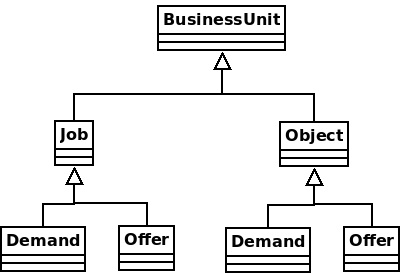
\includegraphics[scale=0.75]{modelsBU2.png}}
\end{center}
\vspace{1cm}

On remarque tout de suite que les classes Offre et Demande sont redondantes et nous avons ainsi une solution peu efficace.  Pour la suite du développement du framework,  il serait intéressant d'abstraire les offres et demandes dans une classe,  par exemple,  Transaction.  Ainsi,  le système réaliserait des échanges de Transactions de BusinessUnits.  Le schéma donnerait ce qui suit : 
\vspace{1cm}
\begin{center}
\fbox{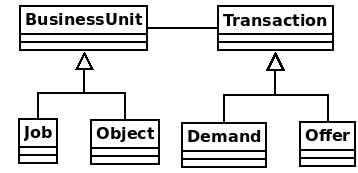
\includegraphics[scale=0.75]{newmodelsBU.png}}
\end{center}
\vspace{1cm}

Ce design permettrait de rendre le framework plus facilement adaptable pour prendre en compte l'existence,  ou non,  d'encoder des offres,  demandes,  concernant des objets ou transactions.  
\vspace{0.5cm}
Cependant,  la mise en place de ce design devrait,  selon moi,  amener un très important refactoring.  A peu près tout le code du fichier views.py (actuellement plus de 1200 lignes de code) devrait être refactoré mais pourrait amener à diminuer le nombre de classes/méthodes nécessaires à la coordination des actions.  Les templates sont également a réorganiser totalement pour pouvoir afficher correctement chaque type de transaction possible.   
\vspace{0.5cm}
 L'étape suivante peut consister en l'ajout de nouveaux features.  La méthode pour y parvenir devrait,  selon moi,  être un développement incrémental,  tel que commencé pour ce projet. En effet,  il est plus facile de suivre la démarche que nous avons décrite dans le chapitre sur le développement et ce,  pour chaque feature un par un.  Ceci semble nécessaire à la vue de la complexité du projet.  
\vspace{0.5cm}
D'une manière de plus globale,  il peut être intéressant d'envisager le concept de communauté de développeurs.  En effet,  ce framework est à destination d'organisations que l'on peut qualifier de ``transitionnaires'' et il a été développé sous licence open-source.  Ainsi,  ce serait une belle opportunité qu'un groupement se crée autour du framework afin d'une part pouvoir soutenir les organisations locales qui désirent instancier le framework,  et d'autre part,  développer de nouveaux features.  Il s'agit là,  selon moi,  d'une piste intéressante pour que ce projet soit utile à la société et utilisé par un maximum de projets locaux.  

